\documentclass[]{usiinfdocprop}
\usepackage{lipsum}
\begin{committee}
  \advisor{Prof.}{Carlo}{Ghezzi}{Politecnico di Milano, Italy}
  \internalmember{Prof.}{Mehdi}{Jazayeri}
  \internalmember{Prof.}{Walter}{Binder}
  \externalmember{Prof.}{Tevfik}{Bultan}{University of California -
    Santa Barbara, USA}
  \externalmember{Prof.}{Schahram}{Dustdar}{Technische Universit\"at  Wien, Austria}
  \externalmember{Prof.}{Sebasti\'an}{Uchitel}{Universidad de Buenos
    Aires, Argentina}
\end{committee}
\phddirector{Prof. Olaf Schenk}
\author{Aryan Eftekhari}
\title{Some Titles}
\subtitle{Second Title}
\usepackage{tikz}
\usetikzlibrary{automata}
\usepackage{listings}

%change 'sl' to 'bf' for bold, or 'normalfont' for no special
%formatting
\captionsetup{labelfont={sl,sf}}

\lstdefinelanguage{algebra}
{morekeywords={import,sort,constructors,observers,transformers,axioms,if,
else,end},
sensitive=false,
morecomment=[l]{//s},
}
\abstract{\lipsum[1]}
\begin{document}
\maketitle
\frontmatter
\tableofcontents
\mainmatter
\chapter[Short title]{Introduction}

\lipsum[2-5]

\begin{figure}
\centering
a figure\dots
\caption{\textsc{Automaton} for something or other. A caption can be rather
long and \emph{should} then consist of complete sentences ended with a `.'}
\end{figure}

\section{The first \textsc{Section}}

Here is some text with \textsc{SmallCaps} in normal font.

\lipsum[6-7]

 \section{The second, math section}
\begin{center}
  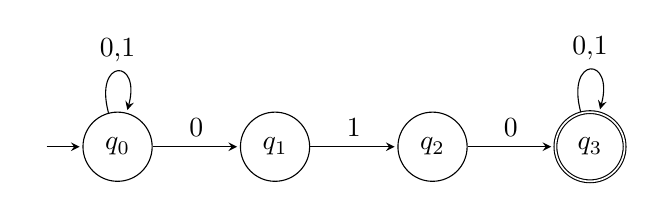
\begin{tikzpicture}[shorten >=1pt,node distance=2cm,auto, initial text=, >=stealth] 
    \node[state, initial] (q0) {$q_0$};
    \node[state] (q1) [right of=q0] {$q_1$};
    \node[state] (q2) [right of=q1] {$q_2$};
    \node[state, accepting] (q3) [right of=q2] {$q_3$};
    \path[->]
    (q0) 
    edge [loop above] node {0,1} ()
    edge  node {0} (q1)
    (q1)
    edge  node {1} (q2)
    (q2)
    edge node {0} (q3)
    (q3)
    edge [loop above] node {0,1} ()
;
  \end{tikzpicture}
\end{center}

\textbf{Theorem 1 (Residue Theorem).}
Let $f$ be analytic in the region $G$ except for the isolated singularities $a_1,a_2,\ldots,a_m$. If $\gamma$ is a closed rectifiable curve in $G$ which does not pass through any of the points $a_k$ and if $\gamma\approx 0$ in $G$ then
\[
\frac{1}{2\pi i}\int_\gamma f = \sum_{k=1}^m n(\gamma;a_k) \text{Res}(f;a_k).
\]
\textbf{Theorem 2 (Maximum Modulus).}
\emph{Let $G$ be a bounded open set in $\mathbb{C}$ and suppose that $f$ is a continuous function on $G^-$ which is analytic in $G$. Then}
\[
\max\{|f(z)|:z\in G^-\}=\max \{|f(z)|:z\in \partial G \}.
\]

\section[third]{A very very long section, titled ``The third section'', with
  a rather  short text alternative (third)}
\lipsum[8-11]
 \texttt{Some Test}
\lstset{language=algebra,linewidth=0.95\linewidth,breaklines=true,numbers=left,
basicstyle=\ttfamily,numberstyle=\tiny,escapeinside={//*}{\^^M},
mathescape=true}
\begin{lstlisting}
import IntSpec, ItemSpec;

sort cart; //*\label{sort}

constructors //*\label{begin-sig}
create() $\longrightarrow$ cart;
insert(cart, item) $\longrightarrow$ cart;
observers
amount(cart) $\longrightarrow$ int;
transformers
delete(cart, item) $\longrightarrow$ cart; //*\label{end-sig}

axioms //*\label{begin-axioms}
forall c: cart, i, j: item 

amount(create()) $=$ 0; //*\label{begin-amount}
amount(insert(c,i)) $=$ amount(c) $+$ price(i); //*\label{end-amount}
delete(create(),i) $=$ create(); //*\label{begin-delete}
delete(insert(c,i),j) $=$
if (i =$\:$= j) c
else insert(delete(c,j),i); //*\label{end-axioms}
end
\end{lstlisting}

Listing taken from~\cite{bg:soswe07}.

\chapter{Second Chapter}
\section{Section One of Two}
\lipsum[8-15]
\section{Section Two of Two}
\lipsum[15-22]

\nocite{*}

\appendix %optional, use only if you have an appendix

\chapter{Some retarded material}
\section{It's over\dots}
\lipsum[22-29]


\backmatter
\bibliographystyle{plainnat}
\bibliography{biblio}

\end{document}

%%% Local Variables: 
%%% mode: latex
%%% TeX-master: t
%%% End: 
